
\documentclass[11pt]{article}
  	\usepackage{ucs} 
	\usepackage[utf8x]{inputenc} % Включаем поддержку UTF8  
	\usepackage[russian]{babel}  % Включаем пакет для поддержки русского языка 
	\usepackage {mathtext}
	\usepackage{amsmath, amssymb}
	\usepackage{graphicx}
	\usepackage{listings}
	\usepackage{hyperref}
	\usepackage{revsymb}
	\hypersetup{
    colorlinks=true,
    linkcolor=blue,
    filecolor=magenta,      
    urlcolor=cyan,
	}
	\urlstyle{same}
	\DeclareGraphicsExtensions{.pdf,.png,.jpg,.jpeg}
	\setcounter{MaxMatrixCols}{20}
	\graphicspath{{pictures/}}
    \title{\textbf{Исследование возможности реализации алгоритма Дойча \\ -- \\ Investigation of the possibility of implementing the Deutsch – Jozsa's algorithm}}
    \author{И.А.Юхновский, Ю.И.Аношкин}
    \date{сентябрь 2020}
    

\begin{document}

\maketitle
\thispagestyle{empty}
\section*{Аннотация}
В статье рассматривается возможность построения квантового алгоритма Дойча на частицах ионизирующего излучения. Демонстрируютя наглядные примеры физических моделей и теоретические обоснования возможности реализации алгоритма в качестве лабораторного эксперимента. Отмечаются перспективы построения квантового компьютера в инфраструктуре объектов ядерного топливного цикла.

\section*{Brief}
The article discusses the possibility of constructing a quantum Deutsch – Jozsa algorithm on particles of ionizing radiation. Was demonstrates examples of physical models and theoretical substantiation of algorithm's implementation as a laboratory experiment. Prospects for building a quantum computer in the infrastructure of nuclear fuel cycle facilities are noted.

\section{Введение}
Алгоритм Дойча ~\cite{Sysoev, Courcera_KvVich} - это определение в один проход функции f(x), из четырех возможных, c целыми аргументами [0,1]: \\

\begin{equation}
F(x) = 
 \begin{cases}
    f(x) = 0 & \text{,}\\
    f(x) = 1 & \text{,} \\
	f(x) = x & \text{,} \\
	f(x) = \overline x \text{.}	   
 \end{cases}
\end{equation}

Для классического случая результат функции F(x) можно записать в табличной форме:

\begin{equation}
\begin{tabular}{|c|c|c|}
\hline
	0 & $f(x) = 0 $ & 0 \\
\hline
	1 & $f(x) = 0 $ & 0 \\
\hline
	0 & $f(x) = 1 $ & 1 \\
\hline
	1 & $f(x) = 1 $ & 1 \\
\hline
	0 & $f(x) = x $ & 0 \\
\hline
	1 & $f(x) = x $ & 1 \\
\hline
	0 & $f(x) = \overline x $ & 1 \\
\hline
	1 & $f(x) = \overline x $ & 0 \\
\hline
\end{tabular}
\end{equation}

Функцию F(x) назовем оракулом.
Рассмотрим как реализовать простейший квантовый компьютер на примере двух оракулов - для заряженных и незаряженных частиц. \\

Будем рассматривать процесс измерения для аргумента $x=1$ (поэтому стенды должны соблюдать поведение F(1), а как они будут вести себя при F(0) - нам неинтересно), поэтому, сделаем упрощение : \\

\begin{equation}
\begin{tabular}{|c|c|c|}
\hline
	1 & $f(x) = 0 $ & 0 \\
\hline
	1 & $f(x) = 1 $ & 1 \\
\hline
	1 & $f(x) = x $ & 1 \\
\hline
	1 & $f(x) = \overline x $ & 0 \\
\hline
\end{tabular}
\end{equation}

В алгоритме Дойча оператор Адамара так нормирует вектора состояний системы, чтобы они не сливались, но в нашем случае полное соответствие этому требованию лишило бы модели наглядности и усложнило бы стенды, поэтому на 0 сигнале мы в некоторых состояниях делали допущения, что они не сливаются.\\

\section{Cтенд №1 - Отражение частиц}

Принципиальная схема стенда : \\


\begin{figure}[htp]
\centering
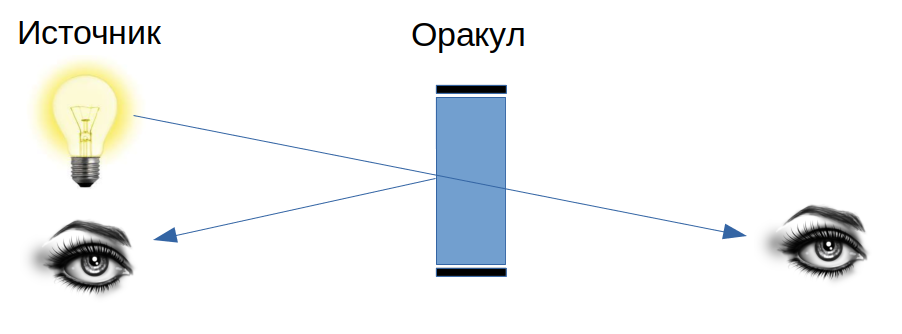
\includegraphics[scale=0.30]{st1.png}
\caption{Схема стенда}
\label{}
\end{figure}

Рассмотрим оракулы и запишем состояние того что видит человек в виде суперпозиции интенсивностей отраженного $I_1$ и прошедшего через оракул $I_2$ света, нормированную к исходной интенсивности $I_0$. Запись состояния системы в виде вектора в нотации дирака |$I_1$ $I_2$> будем называть кубитом. \\

Таким образом, кубит решения задачи Дойча должен соответствовать одной из функций (1), что можно записать следующим образом: \\

\begin{equation}
F(I_0)=|I_1I_2>
\end{equation}


\subsection{$f(x)=0$}
Для этого состояния можно выбрать абсолютно черное тело, тогда кубит этого состояния будет |00> - ничто не отразиться и ничто не пройдет через оракул.

\begin{figure}[htp]
\centering
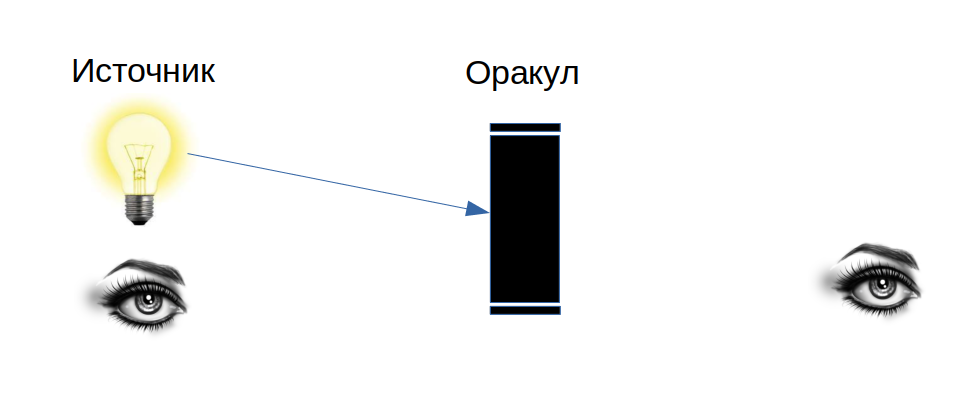
\includegraphics[scale=0.30]{st1_00.png}
\caption{$f(x)=0$}
\label{}
\end{figure}

\subsection{$f(x)=1$}
Для этого состояния оракулом нужно сделать источник света , тогда кубит этого состояния будет |11> - и первый и второй наблюдатель увидят лампочку. 

\begin{figure}[htp]
\centering
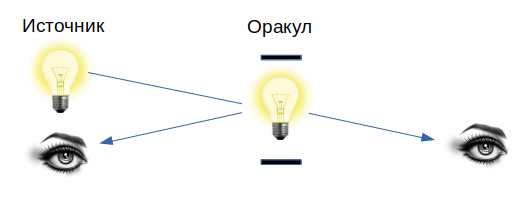
\includegraphics[scale=0.50]{st1_11.png}
\caption{$f(x)=1$}
\label{}
\end{figure}


\subsection{$f(x)=x$}
Для этого состояния оракулом будет пустота, тогда кубит этого состояния будет |01> - второй наблюдатель увидит лампочку. 

\begin{figure}[htp]
\centering
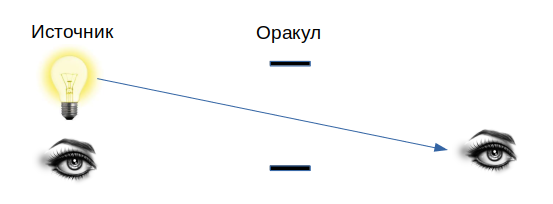
\includegraphics[scale=0.50]{st1_01.png}
\caption{$f(x)=x$}
\label{}
\end{figure}

\subsection{$f(x)=\overline x$ }
Для этого состояния оракулом пусть будет пластина, которая половину интенсивности падающего пучка пропускает, а половину отражает. Тогда, кубит будет |1/2 1/2> 

\begin{figure}[htp]
\centering
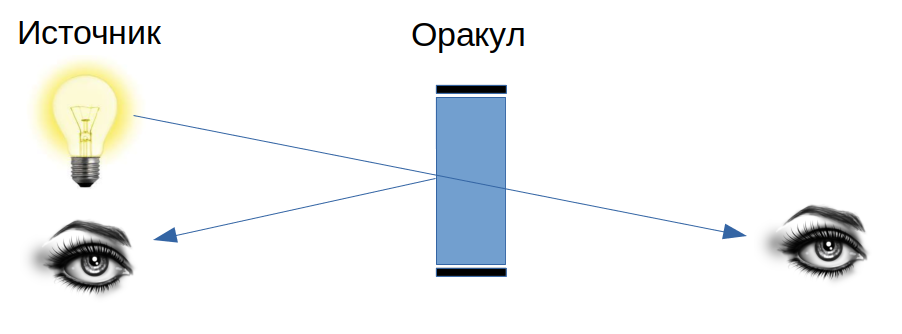
\includegraphics[scale=0.30]{st1.png}
\caption{$f(x)=\overline x$}
\label{}
\end{figure}

\subsection{Соответствие результатов вычислений искомым функциям }

Запишем сводную таблицу для решений:

\begin{equation}
\begin{tabular}{|c|c|c|}
\hline
	1 & $f(x) = 0 $ & |00> \\
\hline
	1 & $f(x) = 1 $ & |11> \\
\hline
	1 & $f(x) = x $ & |01> \\
\hline
	1 & $f(x) = \overline x $ & |1/2 1/2> \\
\hline
\end{tabular}
\end{equation}

Как видим, каждой функции соответствует уникальное значение кубита. Таким образом, задача решается в посылке одного сигнала, вместо классических двух.

\section{Стенд №2 - отклонение и поглощение}

Стенд состоит из лампы, являющейся оракулом, единичного сигнала - электрона и флюоресцентного экрана. \\
 
\begin{figure}[htp]
\centering
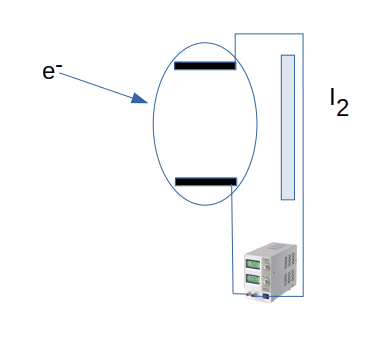
\includegraphics[scale=0.40]{st2.png}
\caption{Стенд №2 отклонение электрона}
\label{}
\end{figure}

На флюоресцентом экране $I_2$ мы будем видеть интенсивности в разных местах, при разных значениях напряжения между анодом и катодом лампы. \\
При отсутствии напряжения электрон продолжит свое движение и упадет на экран в точке $x_0$. \\
При очень высоком напряжении электрон упадет на анод и на экране не будет интенсивности. \\
При невысоком напряжении - отклонится от точки, куда бы он попал без напряжения $x_1$. \\

 Но в такой модели у нас сливаются состояния f(x)=0 и x=0, что недопустимо, поэтому модернизируем стенд \footnote{Лучшей модернизацией было бы применение ловушки Пеннинга, моделирующую макроскопический атом, в котором ядро заменено внешним полем  ~\cite{Ekstrom}, но эта работающая модель более сложная, чем то упрощение, которое мы применим далее. Ловушка Пеннинга будет рассмотрена в отдельной статье.}:

\begin{figure}[htp]
\centering
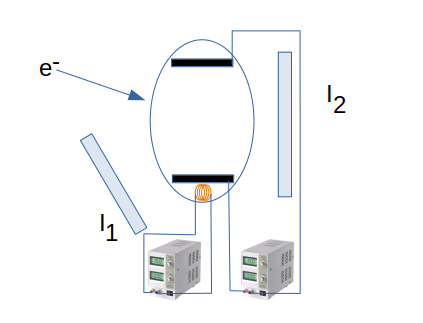
\includegraphics[scale=0.40]{st3.png}
\caption{Стенд №3 отклонение электрона}
\label{}
\end{figure}

В лампу добавим спираль накаливания катода, чтобы катод эмиттировал электроны на анод\footnote{Нам нужно содзать условия для упругого рассеяния. Вместо эмиттирования электронов можно было бы добавить механизм по закачиванию/выкачиванию жидкого водорода. Первые опыты с упругим рассеянием электронов были проведены на цели из жидкого водорода в 1960-1970 годах в Стэнфордской Линейной Ускорительной лаборатории SLAC  с энергией электронов порядка 100МэВ ~\cite{Courcera_KvVich} }. Тогда электрон с некоторой вероятностью (сечением) при сигнале 1 столкнется с эмитированным электроном и отразится на экран $I_1$. А также, лампа может находиться в двух состояниях - катод наверху, катод внизу из-за чего электрон будет отклоняться вверх или вниз на экране $I_2$. \\

Введем нормы для напряжения: \\
0 - нет напряжения \\
1/2 - рабочее напряжение лампы \\
1 - максимальное напряжение лампы \\

Для интенсивности свечения экрана относительно интенсивности излучателя:\\
0 - нет \\
1/2 - отраженная \\
1 - такая же как у источника \\

С учетом трех положений интенсивность на втором экране, вектор состояний системы запишется как |$I_0$ $I_{11}$ $I_{12}$ $I_{13}$> \\

Для $f(x) = 1 $ поместим источник внутрь лампы \\

\begin{equation}
\begin{tabular}{|c|c|c|c|c|}
\hline
	Сигнал & Функция & Напряжение & Положение катода & Вектор состояния \\
\hline
	1 & $f(x)=0 $ & 1 & неважно & |1/2 0 0 0 > \\
\hline
	1 & $f(x) = 1 $ & 0 & неважно & |1 1 1 1 > \\
\hline
	1 & $f(x) = x$ & 1/2 & сверху & |1/2 0 0 1 > \\
\hline
	1 & $f(x) = x$ & 1/2 & снизу & |1/2 1 0 0 > \\
\hline
\end{tabular}
\end{equation}

\section{Одномерное приближение}
Рассмотрим динамику одномерной квантовой системы, описыаемой уравнением Шредингера: \\
\begin{equation}
i\hbar \frac{\partial \psi}{\partial t} = - \frac{\hbar^2}{2m}\frac{\partial^2 \psi}{\partial x^2} + V\psi
\end{equation}
, где $\psi$ - волновая функция частицы, $m$ - масса частицы, $V$ - потенциал квадратного барьера\\

Для решения волнового уравнения воспользуемся преобразованием Фурье  ~\cite{koen}: \\
\begin{equation}
\tilde f(k) = \frac{1}{\sqrt{2\pi}} \int_{-\infty}^{+\infty} e^{-ikx} f(x) dx
\end{equation}
\begin{equation}
\tilde f(x) = \frac{1}{\sqrt{2\pi}} \int_{-\infty}^{+\infty} e^{ikx} \tilde f(k) dk
\end{equation}

Рассчитаем для ширины потенциала равного 0,1,3,10 L, где $L=\frac{\hbar}{2mV_0}$, $V_0$ - потенциал.\\

$a = 0\cdot L$ \\
\begin{tabular}{ccc}
	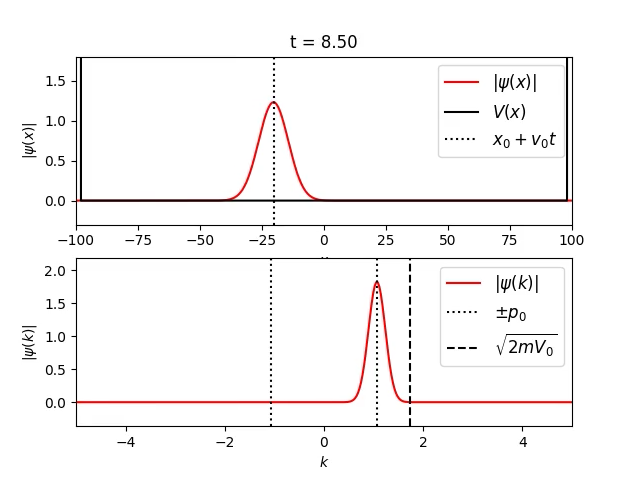
\includegraphics[scale=0.2]{sh_0_8_50} & 
	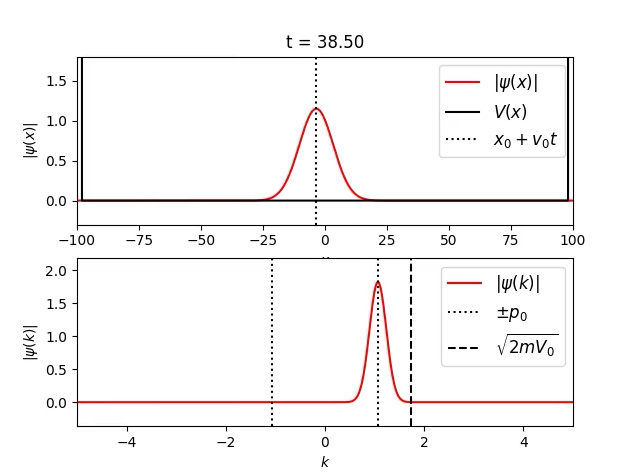
\includegraphics[scale=0.2]{sh_0_38_50} & 
	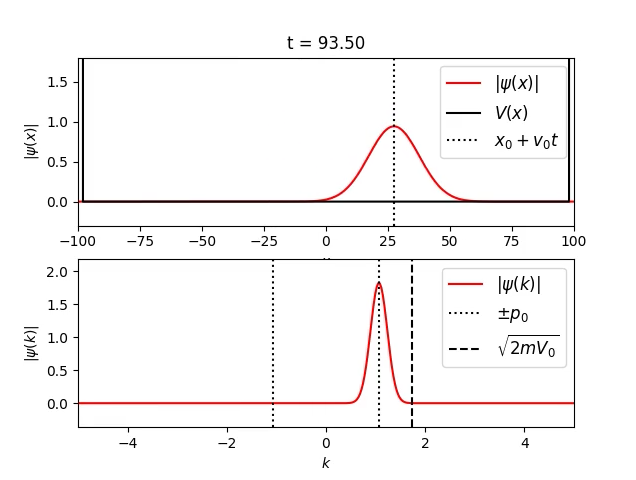
\includegraphics[scale=0.2]{sh_0_93_50} \\
\end{tabular}

$a = 1\cdot L$ \\
\begin{tabular}{ccc}
	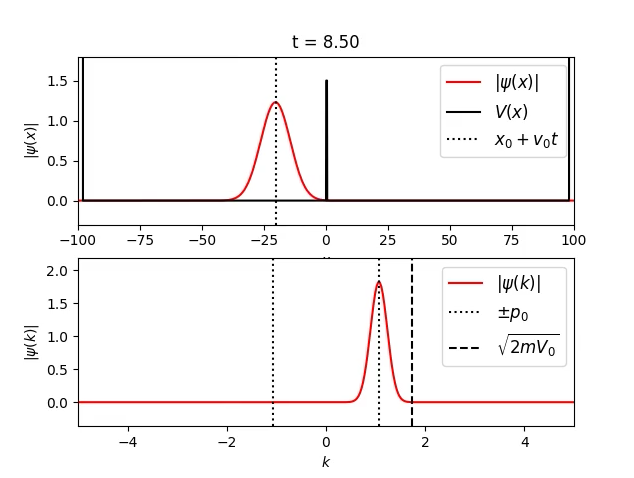
\includegraphics[scale=0.2]{sh_1_8_50} & 
	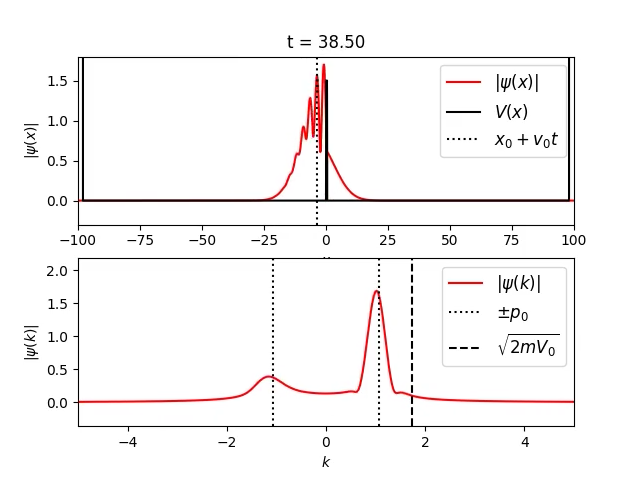
\includegraphics[scale=0.2]{sh_1_38_50} & 
	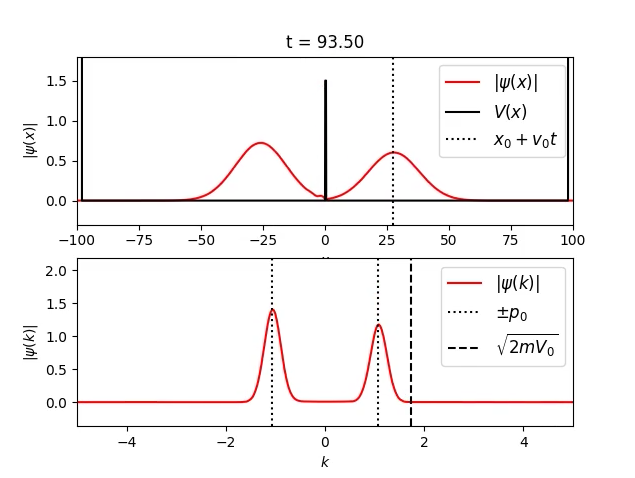
\includegraphics[scale=0.2]{sh_1_93_50} \\
\end{tabular}

$a = 3\cdot L$ \\
\begin{tabular}{ccc}
	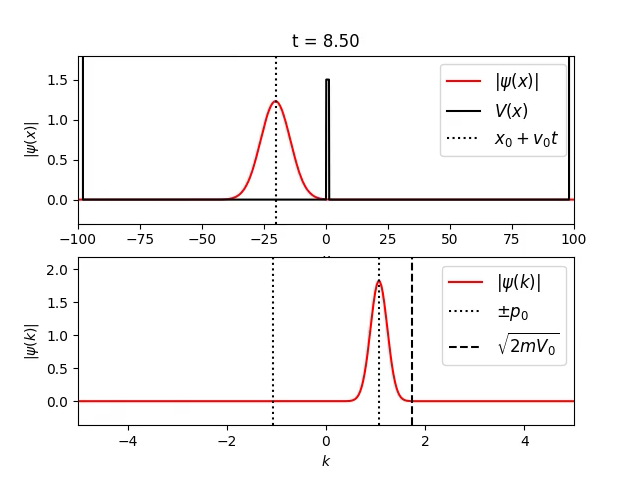
\includegraphics[scale=0.2]{sh_3_8_50} & 
	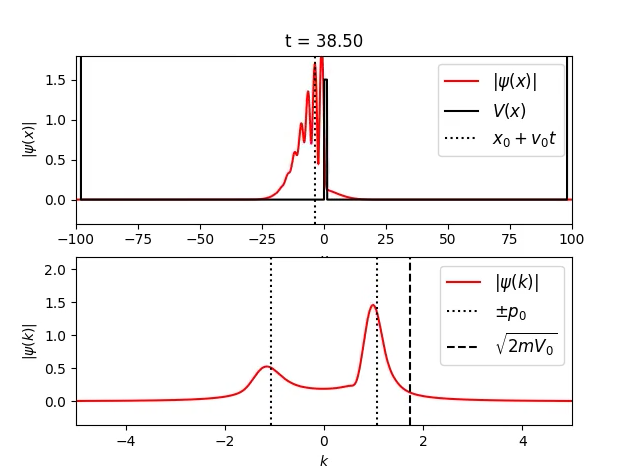
\includegraphics[scale=0.2]{sh_3_38_50} & 
	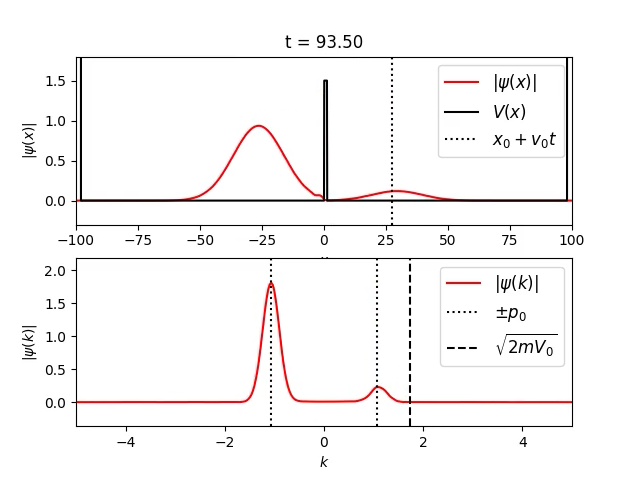
\includegraphics[scale=0.2]{sh_3_93_50} \\
\end{tabular}

$a = 10\cdot L$ \\
\begin{tabular}{ccc}
	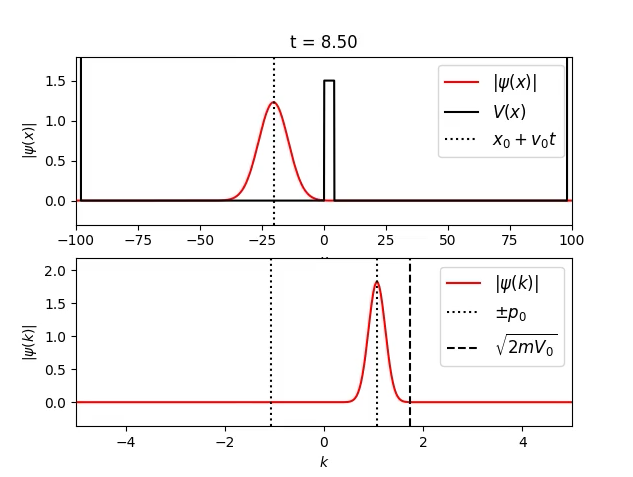
\includegraphics[scale=0.2]{sh_10_8_50} & 
	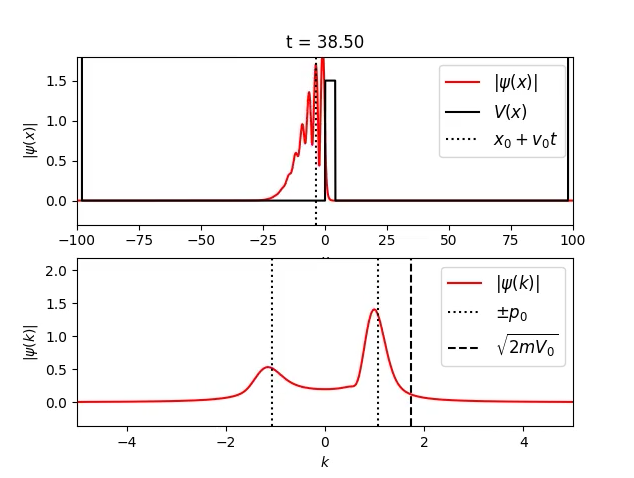
\includegraphics[scale=0.2]{sh_10_38_50} & 
	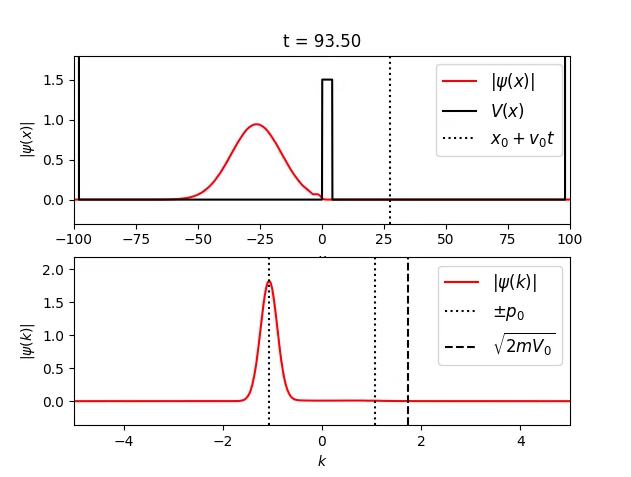
\includegraphics[scale=0.2]{sh_10_93_50} \\
\end{tabular}

Начальные условия для рассчетов могут быть взяты: \\
энергия -  на сайте ОАО <<В/О Изотоп>>\footnote{\url{http://www.isotop.ru/production/}} для различных  источников \\
свойства частиц - particle data group\footnote{\url{https://pdg.lbl.gov/2020/mcdata/mass_width_2020.mcd}}

Таким образом можно подобрать такие потенциалы (и способы управления), при котором поведение волновой функции будет отличаться по времени и на этом принципе реализовать гейты квантового компьютера.

\section{Сечения}
Рассмотренные модели можно обобщить как суперпозиции вероятностных процессов: эластичного и неэластичного рассеяния и поглощения. В ядерной физике это будет хорошо известная функция полного сечения~\cite{Giancoli}: 

\begin{equation}
\sigma_{tot} = \sigma_{el}+\sigma_{inel}+\sigma_{abs}
\end{equation}

По золотому правилу Ферми \cite{Courcera_NPh, Mart} : 
\begin{equation}
W=|M|^2Q
\end{equation}
, где: \\
W - скорость реакции, \\
М - инвариантная амплитуда процесса, \\
Q - плотность квантовых состояний, \\

мы можем записать соответствие между сечением и волновой функцией:
\begin{equation}
d\sigma = \frac{|M|^2}{F}dQ
\end{equation}
где: \\
F - поток, \\
dQ - фактор фазового пространства, учитывающий количество состояний, которые могут быть реализованы конечным состоянием,\\
M - амлитуда вероятности, значения волновой функции. 

Сечение можно определить как вероятность взаимодействия двух частиц путем обмена промежуточным бозоном ( в ~\cite{Martin} приводятся практические примеры, а в ~\cite{Sarycheva} аналитические интерпретации зависимости $\sigma_{tot}(E)$ ).

Действие калибровочного бозона на собственные состояния частицы - есть физическая интерпретация действия оператора на кубит в квантовых вычислениях.

Варианты запутывания частиц могут реализовываться как на одном процессе взаимодействия частиц, так и на некоторой последовательности. 

Отдельно стоит отметить в качестве варианта запутывания - процессы распада частиц. 

Таким образом, зная поток, сечения, волновую функцию частицы мы можем определять dQ (а точнее, составляющую ее функцию  $\delta ^{(4)} $ - обеспечивающую сохранение энергии имульса, а также квантовых состояний для всех частиц в конечном состоянии). Изменяя определенным образом поток, сечение и волновую функцию, мы можем изменять dQ, а значит, реализовывать программу последовательного изменения dQ, т.е. написать программу квантовых вычислений.

\section{Взаимодействия}
В завершении, рассмотрим какой у нас есть инструментарий в виде взаимодействий, на которых, мы можем реализовать наши квантовые операции: 

а) деление; 

б) взаимодействия между заряженными частицами и электронами атома: возбуждение, ионизация, многократное кулоновское рассеяние;

в) между заряженной частицей и ядром: упругое и неупругое рассеяние, тормозное излучение;

г) между фотонами и ядрами: рождение $e^{-}e^{+}$-пар;

д) когерентное излучение заряженными атомами: эффект черенкова, переходное излучение. 

Собраны достаточно обширные данные по сечениям этих взаимодействий на разных частицах и материалах\footnote{\url{https://pdg.lbl.gov/2020/hadronic-xsections/hadron.html}}.

\section{Заключение}

Как было продемонстрировано на предыдущих моделях, возможно подобрать такие условия и нормы, при которых вектора состояний системы - кубиты, не сливаются, а выбор взаимодействий и частиц, на которых можно реализовывать вычисления - теоретически ничем не ограничен. 

У современных квантовых компьютеров есть ряд недостатков, которые делают их реализацию дорогостоящей. Складываются они из обслуживания источника излучения, реализации особых условий протекания физических процессов, на которых строятся вычисления и т.д. 

Видится перспективным исследовать возможность реализации квантового компьютера в инфраструктуре ядерного реактора. Здесь возможны различные синергетические эффекты, а именно: \\
- использование частиц ионизирующего излучения (в реакторе, биологической защите, бассейне выдержки)\\
- экономия энергии на излучателе в мобильных установках\\
- использование совместной инфрастуктуры системы охлаждения\\
- возможность подбора таких параметров взаимодйествующих частиц, для которых несущественны тепловые колебания\\
- возможность использования рекомбинации частиц - аннигиляции и рождения, что может расширять общее количество состояний алгоритма, кубитность системы в целом.

Второе направление, где может быть получен синергетический эффект - использование продуктов переработки ядерного топлива - изотопов, для мобильных квантовых вычислителей. В этом случае источник может быть размещен в непосредственной близости с p-n переходами процессора.

Также, теоретически, интересно рассматреть различные реакции с кварками и их применение в вычислителях. Так для примера рассмотрим реакцию $\beta^{-}$ излучения: $n \rightarrow pe^{-} \overline \nu_e $. В классической реализации на три бита нужно 6 p-n-p переходов (транзисторов), а в ядерной интерпретации все умещается в одну частицу: n=udd переходит в p=udu, что можно представить как |100> $\rightarrow $ |101> а событие регистрируется по появившемуся у частицы электрическому заряду. 

\begin{thebibliography}{3}
\bibitem{Sysoev}
Сысоев С.С. Введение в квантовые вычисления. Квантовые алгоритмы, стр.64 -- СПб.: Издательство Санкт-Петербургского университета, 2020
\bibitem{Courcera_KvVich}
Сысоев С.С. Квантовые вычисления (Quantum computing) -- https://www.coursera.org/learn/kvantovyye-vychisleniya : Санкт-Петербургский государственный университет, 2020
\bibitem{Martin}
B.R.Martin, G.Shaw Particle physics, Third Edition, p.24 -- John Wilye and Sons Ltd, 2008
\bibitem{Courcera_NPh}
Martin Pohl, Anna Sfyrla, Mercedes Paniccia Particle Physics: an Introduction., 4.2 Electromagnetic scattering -- https://www.coursera.org/learn/particle-physics/lecture/Vd0tP/4-2-electromagnetic-scattering Университет Женевы, 2020
\bibitem{Sarycheva}
Л.И.Сарычева Введение в физику микромира. Физика частиц и ядер. стр.66 -- М.: Книжный дом <<ЛИБРОКОМ>>, 2012 
\bibitem{Mart}
Martin Pohl Particles, Fields, Space-Time: From Thomson's Electron to Higgs' Boson -- CRC Press, 2020
\bibitem{Ekstrom}
P.Ekstrom and D.Wineland The Isolated Electorn -- Scientific American, 243, p.90 -- 1980
\bibitem{Giancoli}
Douglas C.Giancoli Physics for Scientists and Engineers with Modern Physics, Fourth Edition, p.1301 -- England: Pearson Education Limited, 2014 
\bibitem{koen}
Клод Коэн-Таннуджи, Бернар Диу, Франк Лалоэ Квантовая механика,Том II, стр.757 -- Екатеринбург: Издательство Уральского университета, 2000 

\end{thebibliography}

\end{document}

